\documentclass[lettersize,journal]{IEEEtran}
\usepackage{amsmath,amsfonts}
\usepackage{algorithmic}
\usepackage{algorithm}
\usepackage{array}
\usepackage[caption=false,font=footnotesize]{subfig}
\usepackage{textcomp}
\usepackage{stfloats}
\usepackage{url}
\usepackage{verbatim}
\usepackage{graphicx}
\usepackage{cite}
\hyphenation{op-tical net-works semi-conduc-tor IEEE-Xplore}
\usepackage{booktabs}
\usepackage{amsmath,amsfonts}
\usepackage{algorithmic}
\usepackage{array}
\usepackage{textcomp}
\usepackage{stfloats}
\usepackage{subcaption}
\usepackage{url}
\usepackage{verbatim}
\usepackage{graphicx}
\usepackage{float}
\usepackage{titlesec}
\usepackage{amsthm}
\usepackage{mathtools}
\usepackage{gensymb}
\usepackage{hyperref}
\usepackage{amssymb}
\usepackage{amsmath}
\usepackage{dsfont}
\captionsetup[figure]{font=footnotesize}

\newcommand{\rEarth}{R_{\oplus}}
\newcommand{\viiva}{\mathop{\Bigg/}}
\newcommand{\sij}[3]{\viiva\limits_{\hspace*{-5mm}{#1}}^{\hspace*{5mm}{#2}}{#3}}
\newcommand{\R}{\mathbb{R}}
\newcommand{\N}{\mathbb{N}}
\newcommand{\B}[1]{\mathbf{#1}}
\newtheorem{theorem}{Theorem}
\newtheorem{corollary}{Corollary}
\newtheorem{lemma}[theorem]{Lemma}
\newtheorem{prop}[theorem]{Proposition}
\newtheorem*{remark}{Remark}

\def\BibTeX{{\rm B\kern-.05em{\sc i\kern-.025em b}\kern-.08em
    T\kern-.1667em\lower.7ex\hbox{E}\kern-.125emX}}
\begin{document}

\title{Order Statistics of the SIR and Interference Cancellation in a Narrow-Beam LEO Uplink}
\author{
  \thanks{The work was supported by the Research Council of Finland Grant 339446.}
   Ilari Angervuori, \IEEEmembership{Student Member, IEEE}  and Risto Wichman, \IEEEmembership{Senior Member, IEEE} \thanks{Ilari Angervuori and Risto Wichman are with the Department of Electrical Engineering, Aalto University, Espoo, 02150, Finland. (email: ilari.angervuori@aalto.fi; risto.wichman@aalto.fi).}
 }

% The paper headers
\markboth{Journal of \LaTeX\ Class Files,~Vol.~1, No.~2, December~2023}%
{Shell \MakeLowercase{\textit{et al.}}: A Sample Article Using IEEEtran.cls for IEEE Journals}

\IEEEpubid{}
% Remember, if you use this you must call \IEEEpubidadjcol in the second
% column for its text to clear the IEEEpubid mark.


\maketitle
\begin{abstract}
We investigate the factorial moment measure of the signal-to-interference ratios (SIR) at the typical low Earth orbit base station (LEO BS) with a narrow Gaussian antenna serving an urban area, with a Gaussian mixture shadowing model. This SIR process is characterized by a Poisson-Dirichlet distribution $\text{PD}(0, \cdot)$, which allows us to derive the density of the factorial moment measure. We analyze the coverage probability at the typical LEO BS receiving the three strongest signals and implement successive interference cancellation (SIC). Our results demonstrate that SIC can notably reduce the variance of the SIR while maintaining robust performance.
\end{abstract}

% Note that keywords are not normally used for peerreview papers.
%% \begin{IEEEkeywords}
%% Low Earth orbit, stochastic geometry, order statistics, interference 
%% \end{IEEEkeywords}


\section{Introduction}

\IEEEPARstart{W}{hile the order statistics} of the signal-to-interference (SIR) and interference cancellation have been studied for terrestrial networks \cite{7305791} by using stochastic geometry, they are yet to be explored in low Earth orbit (LEO) networks. We study the SIR of user equipments (UEs) at the typical LEO base station (BS) by utilizing the narrow-beam LEO uplink system model from \cite{10909705} in an urban environment. We utilize the Gaussian Mixture shadowing model, similar to \cite{modelinguplink} and \cite{9684552}, using the parameters presented in \cite{TR38.811}. The density of the factorial moment measure of the signal-to-total-interference (STIR) process follows a Poisson-Dirichlet distribution PD$(0,\cdot)$ (contrary to PD$(\cdot,0)$ in \cite{7305791}), of which the factorial moment measure is well-known. We derive the joint pdf of the STIR and SIR and study the performance metrics of the three strongest UE signals with and without successive interference cancellation (SIC) schemes. In \cite{10909705}, it was observed that the system parameters optimizing the average throughput, corresponding to mean $\log(2)$ user equipments (UEs) inside a LEO BS $-3$ dB footprint, leads to a high variation in the SIR over the LEO BSs. We demonstrate that the link is more stable with interference cancellation. We show that with the SIC, the number of UEs inside a LEO BS $-3$ dB footprint can be doubled while maintaining the average performance of the strongest UE but profoundly reducing the variance in the SIR. Furthermore, the coverage probability of UEs with less strong signals drastically improves.

\begin{table}
   \captionsetup{size=footnotesize}
   \caption{Principal symbols the values and units in the numerical results. We denote (approximate) proportionality ``$\propto$'' or equality ``$=$'' to a variable. For a dimensional number, we denote the units ``SI'' and ``[non-SI].''}
     \label{table:parameters}
  \begin{center}
    \begin{tabular}{c|p{4.5cm}|p{1.9cm}}
      \toprule
      Symbol& Explanation &Values and units
      \\ 
      \hline 
      $h$ & Receiving LEO BS altitudes. &$1000$ km  \\
%      $G[\cdot]$ &Gaussian antenna gain of a BS.&$\R_+ \rightarrow (0,1)$ \\
      $\alpha$ &Power path loss exponent.& $4$\\
      %% $\Phi\subset \R^2$ &Homogeneous PPP on planar Earth. & $\{(x_i,y_i)\}$ km\\
      %% $\Theta \subset \R^3 $ & Homogeneous PPP on spherical Earth surface of average radius $\rEarth=6378$. &$\{(\rEarth,\phi_i,\varphi_i)\}$\break (km, rad, rad) \\
      $\lambda$ & The density of $\Phi$ and $\Theta$, \textit{i.e.}, the mean number of UEs inside an unit area.&$\{0.83,13.3\} \break 10^{-4}\text{/km}^2$\\
      $\epsilon$& The typical LEO BS elevation angle w.r.t $\textit{o}$.&$\left({\pi}/{2},{\pi}/{6}\right)\text{ rad}\break=(90,30)[\degree]$\\
      %% $\kappa$  & Average number of  the LEO BS $-3 \text{ dB footprints};$& \\
      %% ${\tilde{\kappa}}$ &  $\kappa/\log(2)$.& \\
      $p_{\text{LoS}}$& LoS probability; $p_{\text{LoS}} \propto \sin(\epsilon)$. & $(0.992,0.493)$\\
%      $p_{\text{NLoS}}$& NLoS probability; $1-p_{\text{LoS}}$. & \\
      $\mu_{\text{LoS}}$& Mean of the LoS component of the Gaussian mixture shadow fading model. & $0$ [dB] \\
      $\mu_{\text{NLoS}}$& Mean of the NLoS component. & $-26$ [dB] \\
      $\sigma^2_{\text{LoS}}$& Variance of the LoS component. & $4^2$ [dB] \\
      $\sigma^2_{\text{NLoS}}$& Variance of the NLoS component. & $6^2$ [dB] \\
      %% $H_{\mathcal{M}\mathcal{L}\mathcal{N}}$ & A r.v. distributed according to a two-tier $\{\text{LoS}, \text{NLoS}\}$ log-normal mixture distribution representing the power fading.&   \\
      %% $H_{\text{Exp}}$ & A simple approximation of (mean normalized) $H_{\mathcal{M}\mathcal{L}\mathcal{N}}$. It has a defective exponential cdf entirely characterized by the atomic prob. measure at $0$; $1-\upsilon$.&\\
      %% $\upsilon$ & $\mathbb{P}(H_{\text{Exp}}>0)$ $=1-\mathbb{P}(H_{\text{Exp}}=0)$; $\upsilon = \upsilon(p_{\text{LoS}}(\epsilon))=v(\epsilon)$. &$(0.85,0.53)$ \\
      %% $\kappa \upsilon$ & The mean number of effective UEs inside the $-3$ dB footprints. \textbf{The parameter determines the theoretical SIR performance.}&$ \{1.8,2.6\}$ \\
      $\varphi_{\text{RX}}$ & Half-width of the $-3$ dB antenna gain.&$0.028= 1.6 [\degree] \hfill $ \\      
      $\kappa$& Average number of UEs inside a $-3$ dB footprint; $\kappa =\pi \lambda \left({\varphi_{\text{RX}}}h/{\sin^2(\epsilon)}\right)^2$.& $(1.63,6.51)$ \\
      $\upsilon$&Fraction of effective UEs; $\upsilon \propto \sin(\epsilon)$. &$(0.85,0.426)$ \\      
      $\kappa \upsilon$& Average number of effective UEs inside a $-3$ dB footprint.& $\{2,4\}\times \log(2)$ \\
      $\theta$ & SIR threshold of a uccessful transmission.&$(0.2,10)=\hfill$  \break  $(-7,10) \text{ [dB]}$ \\
      $\tau$ & SIR threshold of a successful interference cancellation.& $0.2=\hfill$\break $-7\text{ [dB]}$\\
     % $K$ & Maximum number of interference cancellation cycles in the ASIC\\
     \bottomrule
    \end{tabular}
  \end{center}
\end{table}   





\section{System model}



\begin{figure}[h]%
  \centering
  \subfloat[\centering  Interpretation of the \textit{planar} system model with the satellites in adjacent orbits serving an urban area and a realization of the UEs. The altitudes are not to scale.]{{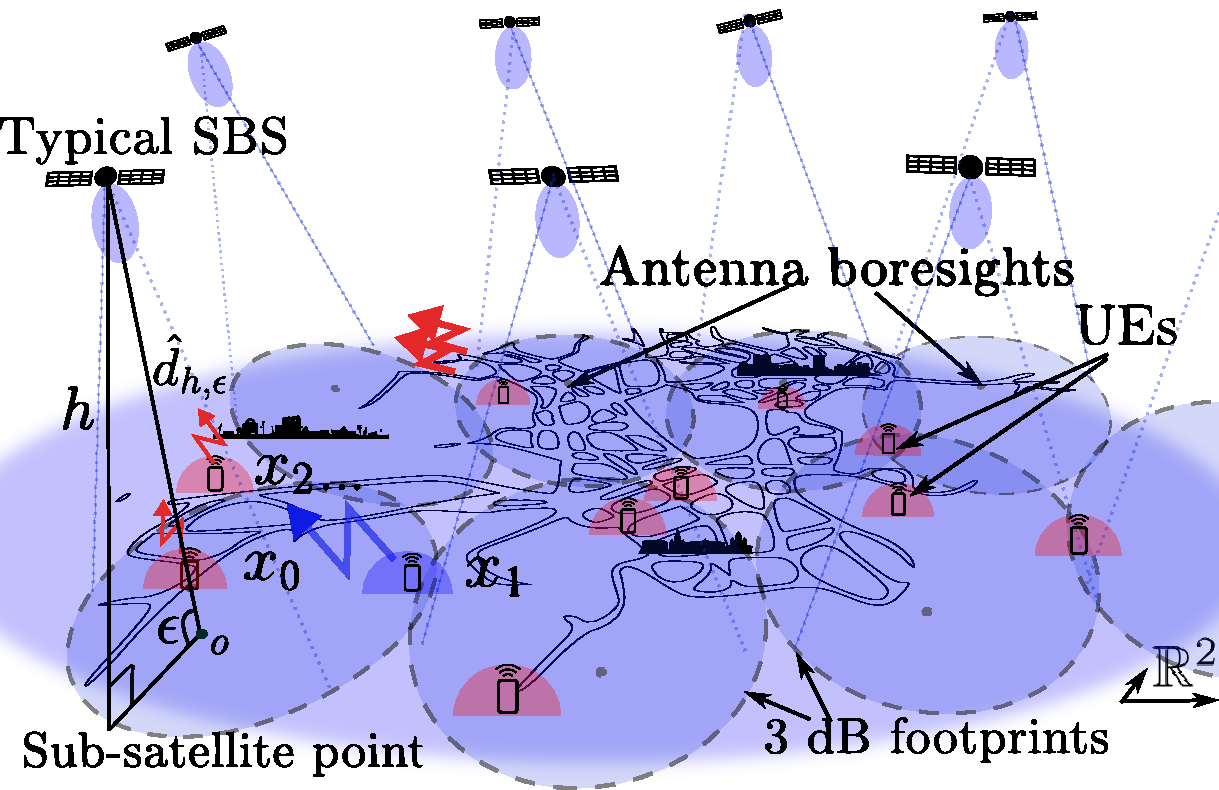
\includegraphics[width=\linewidth]{UEsontheplane2.pdf}}
    \label{fig:UEsontheplane}%%
  } 
  \qquad
  \subfloat[\centering The typical LEO BS as seen from the side. The transmitters are projected into line $(0, \infty)$ according to their norm.]{{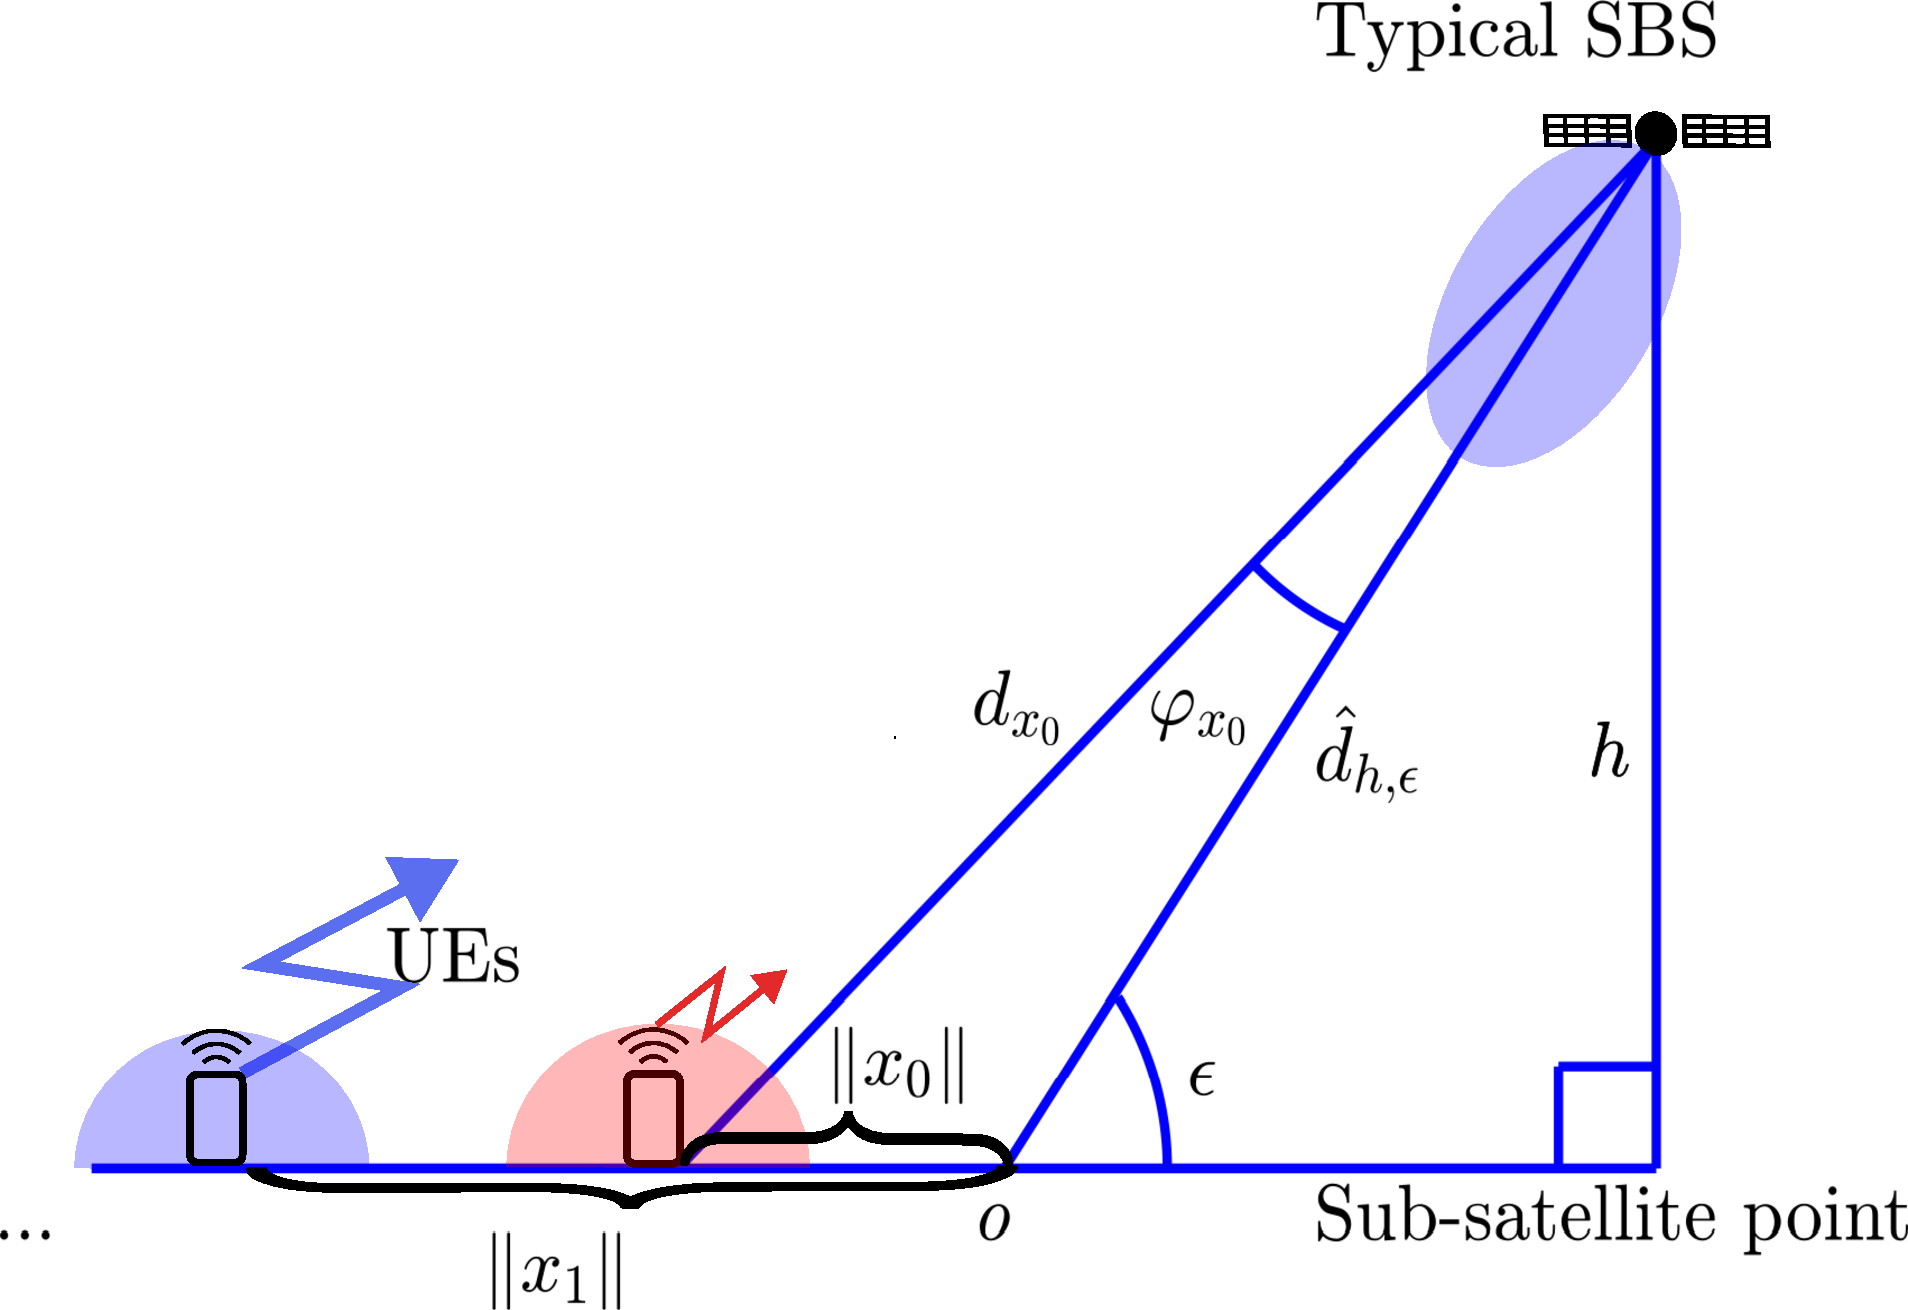
\includegraphics[width=\linewidth]{systemmodel2.pdf}}     \label{fig:systemmodel}} %%
  \caption{The simplified narrow-beam LEO uplink system model. The satellite antenna boresight is oriented towards $\textit{o}$, the focus point of the elliptical footprint. The omnidirectionally transmitting UEs $\{x_i\}$ are located according to the homogeneous PPP on the plane. The transmitter with the strongest signal is the first-served UE.}
\end{figure}




\label{sec:analysissec}






A narrow-band LEO  uplink is considered. The UEs follow a homogeneous PPP $\Phi \subset \R^2$ of density $\lambda$. The LEO BSs form a homogeneous point process (p.p.) possibly with a different density than the UEs. Because of the translation invariancy of the PPP, all locations are statistically equivalent, and we define the origin $\textit{o}$ to represent \textit{the typical LEO BS} footprint focus point.


The path loss, representing the antenna gain at the typical LEO BS, is given over the planar distance $r \in [0, \infty)$ as a Gaussian function
  \begin{equation}
    \label{eq:Gaussianantpat}
    G(r) = 2^{-(D_{h,\epsilon}r)^2 / \varphi_{\text{RX}}^2}.
  \end{equation}
  The angle $\varphi_{\text{RX}}$ denotes the $-3$ dB antenna gain width. Furthermore, the scaling constant $D_{h,\epsilon} \triangleq \sin^2(\epsilon)/h$ is a first-order coefficient of the Taylor expansion of the angle $\varphi_r$ w.r.t. the boresight of the typical antenna pattern. (Thorough details in \cite{10909705}.) %% This is a sufficient approximation for small $r$, for example, for UEs within the main lobe in case of narrow beams characterozed by small $\varphi_{\text{RX}}^2$. Otherwise, because of the fast decay of the Gaussian path loss, the power from the UES with large $r$ practically vanishes.


  %% \begin{remark}[Terrestrial millimeter communication]
  %%   The Gaussian, \textit{i.e.}, the squared exponential (along with other exponential functions) spatial path loss function have applications in terrestrial networks that pose rapid signal attenuation, such as millimeter wave cellular networks in dense urban environments for the NLoS signals [CITE]. Hence, the analysis presented in the paper can be applied to such planar Poisson network models. To the best of our knowledge, similar exploration of the factorial measures has not been conducted with the exponential path loss.  Notably, the squared power term $r^2$, as in the Gaussian function, is particularly tractable compared to other powers. 
  %% \end{remark}

  
  \subsection{Shadowing}

         %%    \begin{figure}[h]%
         %%   \centering
         %%   \subfloat[\centering The average total received power for the path loss exponent $\gamma =2$ as a function of altitude $h$.%is approximately independent of the altitude. 
         %%   ]{{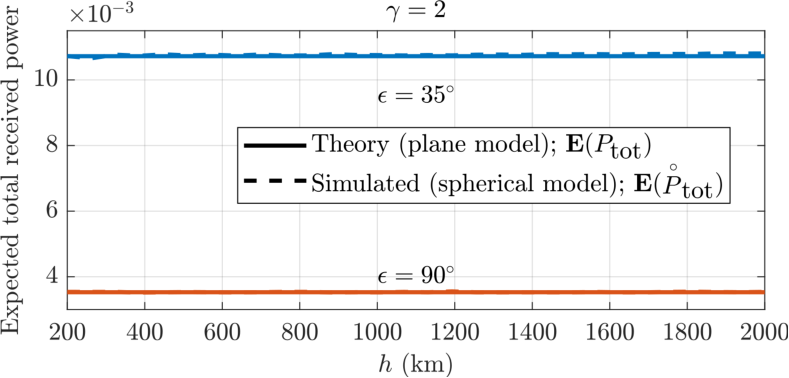
\includegraphics[width=\linewidth]{gamma2means.pdf}}
         %%     \label{fig:gamma2means}%%
         %%   } 
         %%   \qquad
         %%   \subfloat[\centering The average total received power for the path loss exponent $\gamma =4$ as a function of elevation angle $\epsilon$.
         %%   %is approximately independent of the elevation angle. 
         %%   ]{{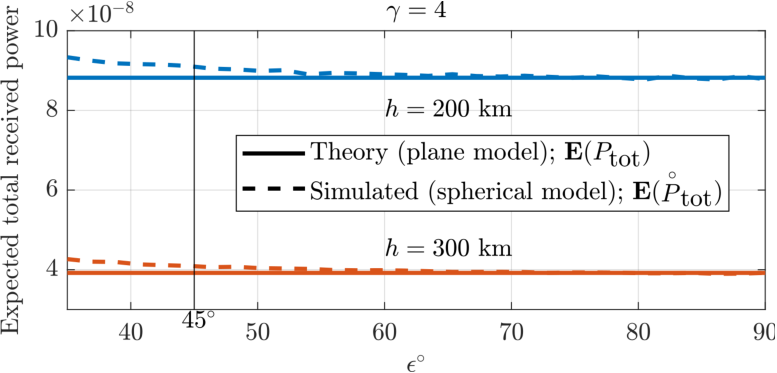
\includegraphics[width=\linewidth]{gamma4means.pdf}}     \label{fig:gamma4means}} %%
         %%   \caption{Comparison of the expected total received power based on the simulated spherical model and the theoretical planar model. 
         %%   %The theory and the simulated spherical model values are compared. 
         %%   The parameters $\varphi_{\text{RX}} = 1.6 \degree, P =1, \lambda =1/\text{km}^2,\gamma \in \{2,4\}, h \in [200,2000] \text{ km}, \epsilon \in  [35\degree,90\degree] $ are used.}
         %% \end{figure}



\subsubsection{Gaussian mixture shadowing model}
\label{sec:guassianmixture}

Consider a two-tier $\{\text{LoS},\text{NLoS}\}$ (line-of-sight and non-line-of-sight) Gaussian mixture shadow fading model with the parameters $\mu_{\text{LoS}} = 0$ dB, $\sigma_{\text{LoS}} = 4$ dB, $\mu_{\text{NLoS}} = -26$ dB, and $\sigma_{\text{NLoS}} = 6$ dB, which correspond to an urban environment \cite{TR38.811}. Assuming i.i.d. power shadow fading for all UEs, \textit{the typical shadowed transmit power} $H_{\mathcal{M}\mathcal{L}\mathcal{N}}$ follows a log-normal mixture distribution;
\begin{align}
  \label{eq:tier2lognormal}
  H_{\mathcal{M}\mathcal{L}\mathcal{N}} &\sim p_{\text{LoS}} \mathcal{L}\mathcal{N}(\rho \mu_{\text{LoS}}, (\rho \sigma_{\text{LoS}})^2) \nonumber \\
  &\quad + p_{\text{NLoS}} \mathcal{L}\mathcal{N}(\rho \mu_{\text{NLoS}}, (\rho \sigma_{\text{NLoS}})^2),
\end{align}
where $p_{\text{LoS}}=1-p_{\text{NLoS}}$ is the LoS probability as in Figure \ref{fig:upsilonvsepsilon}. Considering a natural base for the log-normal distribution, the constant $\rho \triangleq \log(10)/10$ normalizes the parameters $\mu_{\text{LoS}}, \sigma_{\text{LoS}}, \mu_{\text{NLoS}},$ and $\sigma_{\text{NLoS}}$, ensuring that the conditioned r.v.'s $10 \log_{10}(H_{\mathcal{MLN}}|\text{LoS})$ and $10 \log_{10}(H_{\mathcal{MLN}}|\text{NLoS})$ evaluate to r.v.'s following the normal distributions $\mathcal{N}(\mu_{\text{LoS}}, \sigma_{\text{LoS}}^2)$ and $\mathcal{N}(\mu_{\text{NLoS}}, \sigma_{\text{NLoS}}^2)$, respectively.



\subsubsection{Defective exponential shadowing distribution}
As a compromise between analytical tractability and realism, we introduce a \textit{defective} exponential power fading distribution for the UEs, described by the distribution function
\begin{equation}
  \label{eq:defexp}
  F_{{H}_{\text{Exp}}}(t) = \upsilon e^{-t}, t>0.
\end{equation}
Essentially, this is a mixture distribution. Namely, $0 \leq 1-\upsilon < 1$ denotes the probability that the shadowed signal is entirely attenuated and takes the value of zero, otherwise, the power follows the exponential distribution. 

 We introduce a scaling term, $\Upsilon$, to ensure that the means of the log-normal mixture distribution and the defective exponential distribution match: $\mathbb{E}(\Upsilon H_{\mathcal{MLN}}) = \mathbb{E}(H_{\text{Exp}}) = \upsilon$. By equating the first two moments of $H_{\text{Exp}}$ (l.h.s.) and $\Upsilon_{} H_{\mathcal{M} \mathcal{L}\mathcal{N}}$ (r.h.s.)
\begin{equation}
  \label{eq:matchingmoments}
  \begin{cases}
    &\upsilon_{} = \Upsilon_{} \left(p_{\text{LoS}} e^{\mu_{\text{LoS}} + \sigma_{\text{LoS}}^2/2} + p_{\text{NLoS}} e^{\mu_{\text{NLoS}} + \sigma_{\text{NLoS}}^2/2}\right)\\
    &2\upsilon_{}= \Upsilon_{}^2 \left( p_{\text{LoS}} e^{2(\mu_{\text{LoS}} + \sigma_{\text{LoS}}^2)} + p_{\text{NLoS}} e^{2(\mu_{\text{NLoS}} + \sigma_{\text{NLoS}}^2)} \right), 
  \end{cases}
\end{equation}
 we can solve for the parameter $\upsilon$:
\begin{align}
  \label{eq:upsilon}
  & \upsilon_{}=\frac{ 2\left( p_{\text{LoS}}e^{\mu_{\text{LoS}}+\sigma^2_{\text{LoS}}/2}+p_{\text{NLoS}}e^{\mu_{\text{NLoS}}+\sigma^2_{\text{NLoS}}/2} \right)^2}{p_{\text{LoS}}e^{2(\mu_{\text{LoS}}+\sigma_{\text{LoS}}^2)}+p_{\text{NLoS}}e^{2(\mu_{\text{NLoS}}+\sigma_{\text{NLoS}}^2)}}.
    %% \label{eq:Upsilon}
    %% &\Upsilon_{} = \frac{2\left(p_{\text{LoS}}e^{\mu_{\text{LoS}}+\sigma^2_{\text{LoS}}/2}+p_{\text{NLoS}}e^{\mu_{\text{NLoS}}+\sigma^2_{\text{NLoS}}/2}\right)}{p_{\text{LoS}}e^{2(\mu_{\text{LoS}}+\sigma_{\text{LoS}}^2)}+p_{\text{NLoS}}e^{2(\mu_{\text{NLoS}}+\sigma_{\text{NLoS}}^2)}}.
\end{align}
The parameter $\upsilon=\upsilon(\epsilon)$ varies with the elevation angle, influencing the shadow fading characteristics. The parameter $\Upsilon_{}$ holds no significance in an interference-limited scenario, as the equal scaling of all UE powers neutralizes its effect.




\begin{remark}
  The variable $0 < \upsilon \leq 1$ is not generally solvable for all log-normal distribution parameters (by matching the first two moments). Broadly said, the variance of the shadowing has to be large enough. However, the variable $0<\upsilon \leq 1$ is solvable for almost every shadowing scenario in \cite{TR38.811}, particularly for the urban scenario.
\end{remark}

\subsection{The spherical Earth model in the Monte Carlo simulations }

\label{sec:sphericalmodel}
The planar model approximates the spherical system model, where the UEs are located on the spherical Earth surface of radius $\rEarth= 6378$ km according to a homogeneous PPP $\Theta$ of density $\lambda$ represented in spherical coordinates. This p.p. can be constructed from $\Phi \subset \R^2$ by a preserving mapping. Namely, for $x=(x_1,x_2) \in [-\pi,\pi]\times[-1,1]\cap\Phi/\rEarth$,
\begin{align}
  &(x_1,x_2)\mapsto (\rEarth,x_1,\sin^{-1}(x_2))=(\rEarth,\theta_{x_1},\vartheta_{x_2}) \in \Theta.
\end{align}

The total interference at the typical LEO BS from the UEs in the PPP $\Theta \cap E $, with $E$ denoting the area above the horizon of the typical LEO BS, is defined as
\begin{equation}
  \label{eq:mathringptot}
  \mathring{I} \triangleq  \sum_{x \in \Theta \cap E }  \frac{{H_{\mathcal{M}\mathcal{L}\mathcal{N}}}_x G(\varphi_x)}{(d_x/d_0)^{\alpha}},
\end{equation}
where $d_0$ is a normalizing constant. \textit{The simulated values are based on the spherical model}, the angle $\varphi_x$ and distance $d_x$ calculated precisely for each $x \in \Theta \cap E$, \textit{and accurate i.i.d. Gaussian mixture shadowing} ${H_{\mathcal{M}\mathcal{L}\mathcal{N}}}_x$.

\section{Analysis}
For a more detailed analysis and planar model comparison to the spherical model, please refer to \cite{10909705}.
         
Given i.i.d. shadowing variables $\{H_x\}_{x \in \Phi}$, we define the process of the received signal powers at the typical location, referred to as the gain process (GP), by
\begin{equation}
  \label{eq:gainprocess}
  \mathcal{G} \triangleq \left\{ H_x G(\|x\|) : x \in \Phi \right\},
\end{equation}
where $\|x\|$ is the Euclidean distance from $\textit{o}$. 

The GP is a \textit{projection process} mapping the points from $\mathbb{R}^2$ into $(0,\infty)$ and, as such, forms a nonhomogeneous PPP \cite[Section 4.2.5]{alma998193414406526}.



Since the variables $\{H_x\}_{x \in \Phi}$ are i.i.d., we can denote the typical shadowing variable simply as $H$ without the subscript.
\begin{prop}[Density of the GP]\
  Let $F_H(\cdot)$ be the (possibly degenerate) complementary cumulative distribution function (ccdf) of a fading variable $H$. The density function of $\mathcal{G}$ is given by
  \begin{equation}
    \label{eq:GPdensity}
    \lambda_{\mathcal{G}}(t) = \tilde{\kappa} {F_H(t)}/{t}, \quad t \in (0, \infty),
  \end{equation}
  where $\tilde{\kappa} = {\kappa}/{\log(2)}$ and
  \begin{equation}\kappa \triangleq \pi \lambda \left(\frac{\varphi_{\text{RX}}h}{\sin^2(\epsilon)}\right)^2
    \label{eq:kappa}
  \end{equation}
  is approximately the average number of UEs inside a $-3$ dB footprint.

  
  \begin{proof}
    Let $f_H(\cdot)$ be the pdf of $H$. Denote $G^{-1}(\cdot)$ as the generalized inverse of $G$, defined as $G^{-1}(y) = \inf \{x : G(x) < y\}$. According to \cite[Eq. 4.55]{alma998193414406526},
    \begin{align*}
      &\int_t^{\infty} \lambda_{\mathcal{G}}(y) \, dy = \pi \lambda \mathbb{E}\left[ \left({G^{-1}(t/H)}{}\right)^2 \right] \\
      &= \pi \lambda \int_t^{\infty} \left(-\frac{\varphi_{\text{RX}} \sqrt{-\log(t/h)}}{D_{h,\epsilon} \sqrt{\log(2)}}\right)^2 f_H(h) \, dh \\
      &= -\tilde{\kappa} \int_t^{\infty} \log(t/h) f_H(h) \, dh \\
      &\overset{(a)}{=} -\tilde{\kappa} \left[ \left. \log(t/h) F_H(h) \right|_t^{\infty} + \int_t^{\infty} \frac{F_H(h)}{h} \, dh \right].
    \end{align*}
    In (a), we use integration by parts. The result follows by differentiating with respect to $t$ and applying the negative sign. Note that a necessary condition for this procedure is that $\int_t^{\infty} \log(t/h) f_H(h) \, dh$ converges for all $t > 0$.
    
    Please refer to \cite[Lemma 1]{10909705} for throughout explanation of the interpretation of $\kappa$.
  \end{proof}
\end{prop}





The total interference, or total received power, is defined as the sum of the GP at the footprint location  $\textit{o}$ of the typical LEO BS:
\begin{equation}
  \label{eq:totpow}
  I \triangleq \sum_{x \in \Phi} H_x G(\|x\|) = \sum_{x \in \mathcal{G}} x.
\end{equation}


The mean and the variance of $I$ are respectively given by
\begin{align}
  \label{eq:totmean}
  &\mathbb{E}\left(I \right) = \int_{0}^{\infty} t\lambda_{\mathcal{G}}(t) dt = \tilde{\kappa} \int_{0}^{\infty}F_H(t) dt =\tilde{\kappa} \mathbb{E}(H),
\end{align}
and
\begin{align}
  \label{eq:totvar}
  &\text{Var}\left(I \right) = \int_{0}^{\infty} t^2\lambda_{\mathcal{G}}(t) dt= \tilde{\kappa} \int_0^{\infty}tF_H(t) dt  \nonumber \\
  &= \tilde{\kappa} \frac{\text{Var}(H) + \mathbb{E}(H)^2}{2} = \tilde{\kappa}  \mathbb{E}[H^2]/2.
\end{align}

Note that matching the first two moments of the fading distributions \eqref{eq:tier2lognormal} and \eqref{eq:defexp} is equivalent to matching the mean and the variance of the total interference.





          \begin{figure}[h]%
           \centering
           \subfloat[The density of the GP for $\kappa \upsilon \in \{2 \log(2), 4 \log(2)\}$ using $\epsilon = \pi/2$. Interestingly, the elevation angle did not have visible effect on the density in the Gaussian mixture model. ]{{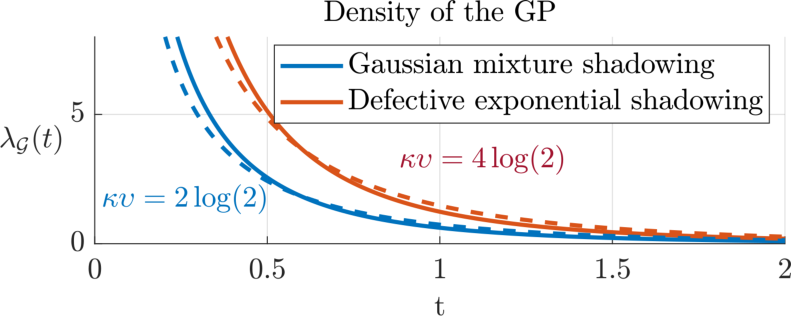
\includegraphics[width=\linewidth]{plotdensities.pdf}}
             \label{fig:densities}}
           \hfil
           \subfloat[The dependence of the shadowing parameters $p_{\text{LoS}}$ and $\upsilon$ on the elevation angle. The parameters are approximately proportional to the sine function. ]{{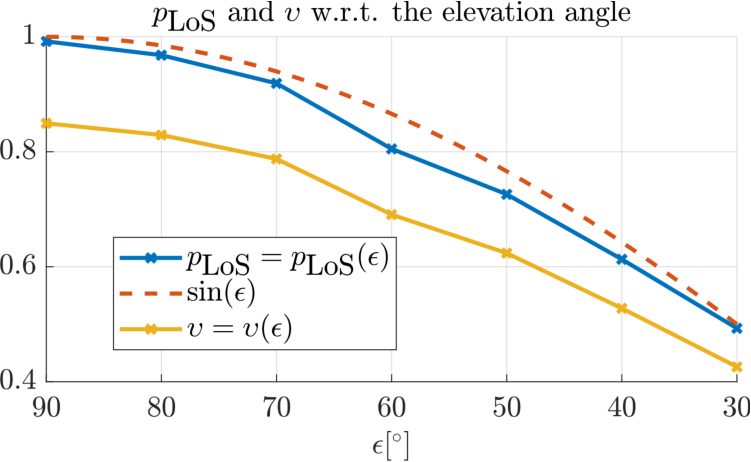
\includegraphics[width=\linewidth]{upsilonvsepsilon.pdf}}     \label{fig:upsilonvsepsilon}} %%
           \caption{The density of the GP and shadowing parameters in the Gaussian mixture and defective exponential shadowing models.}
         \end{figure}









%% The spatial path loss is of no interest in the definition of $I$ because we assume that the spatial path loss is a constant due to the narrow-beam antenna pattern decaying fast to $0$, $G(\cdot)$, which ensures that the relevant UEs are located near one another (see Section \ref{sec:numericalresultsandconnectiontoLEO}). Hence, given that the spatial path loss is identical for all transmitters, it does not influence the SIR. For the SINR, the noise variable can be scaled appropriately to account for the spatial path loss appropriately. 







%% \subsection{Slow-fading distribution}
%% While analytically tractable, the defective exponential distribution can capture the mean and the variance of a more complicated fading distribution with high variance, particularly the lognormal distribution, which is a well-established shadowing model in the LEO networks. The shadowing is defined by the mixed exponential RV
%% \begin{equation}
%%   \hat{H}_x \sim
%%   \begin{cases}
%%     0, \text{ if } U < 1-\rho,\\
%%     \text{Exp}(\mu), \text{ if } U \geq1- \rho,              \label{eq:tier2exponential}
%%   \end{cases}
%% \end{equation}
%% with $\mu>0$ and $0<\rho\leq1$, and $U \sim U(0,1)$ follows the uniform distribution.


%%where
%% \begin{align}
%%   &a=\frac{2 (p_{\text{LoS}}-1) e^{{\mu_{N\text{LoS}}}+\frac{{\sigma_{N\text{LoS}}}^2}{2}}-2 p_{\text{LoS}} e^{{\mu_{\text{LoS}}}+\frac{{\sigma_{\text{LoS}}}^2}{2}}}{(p_{\text{LoS}}-1) e^{2 \left({\mu_{N\text{LoS}}}+{\sigma_{N\text{LoS}}}^2\right)}-p_{\text{LoS}} e^{2 \left({\mu_{\text{LoS}}}+{\sigma_{\text{LoS}}}^2\right)}},\\
%%   &b=\frac{2 \left(({p_\text{LoS}}-1) e^{{\mu_{\text{N\text{LoS}}}}+\frac{{\sigma_{\text{N\text{LoS}}}}^2}{2}}-{p_\text{LoS}} e^{{\mu_{\text{LoS}}}+\frac{{\sigma_{\text{LoS}}}^2}{2}}\right)^2}{({p_\text{LoS}}-1) e^{2 \left({\mu_{\text{N\text{LoS}}}}+{\sigma_{\text{N\text{LoS}}}}^2\right)}-{p_\text{LoS}} e^{2 \left({\mu_{\text{LoS}}}+{\sigma_{\text{LoS}}}^2\right)}}.              
%% \end{align} 



\subsection{Laplace transform of the total received power}

With defective exponential shadowing ${H}_{\text{exp}}$, for Re$(s)>1$,

\begin{align}
  \label{eq:lapdef}
  &\mathcal{L}_{I}(s)\triangleq \mathbb{E}\left(e^{-sI}\right)= \exp\left\{-\int_0^{\infty}(1-e^{-sr}) \lambda_{\mathcal{G}}(r) dr \right\} \nonumber \\
  &=\exp\left\{-\tilde{\kappa}\int_0^{\infty}(1-e^{-sr}) F_{{H}_{\text{exp}}}(r) /r dr \right\} \nonumber \\
  &=\exp\left\{-\tilde{\kappa}\upsilon_{}\int_0^{\infty}(1-e^{-sr}) e^{-r} /r dr \right\} =(1+s)^{-\tilde{\kappa}\upsilon_{}},
\end{align}
which is the Laplace transform of the gamma distribution with the shape parameter $\tilde{\kappa}\upsilon_{}$. 



%% \subsection{STIR process its factorial moment measures}
%%  We denote the signal-to-interference-plus-noise ratio (SIR) process of the UEs as
%% \begin{align}
%%   \label{eq:SINR}
%%   \Psi &= \{\mathsf{Z}: \mathsf{Z} \in \Psi\} \triangleq \left\{ \frac{u}{I-u} : u \in \mathcal{G}\right\} \nonumber \\
%%   &=\left\{ \frac{H_x G(D_{h,\epsilon}\|x\|)}{I-H_x G(D_{h,\epsilon}\|x\|)} : x \in \Phi\right\},
%% \end{align}
%% where $I$ is defined in \eqref{eq:totpow}. Similarly, the signal-to-total-interference ratio (STIR) process is defined as
%% \begin{align}
%%   \label{eq:STINR}
%%   \Psi' &= \{\mathsf{Z}': \mathsf{Z}' \in \Psi'\} \triangleq \left\{ \frac{u}{I} : u \in \mathcal{G}\right\}.
%% \end{align}
%% We can always recover on process from another
%% \begin{equation}
%%   \Psi = \left\{ \frac{\mathsf{Z}'}{1- \mathsf{Z}'}: \mathsf{Z}' \in \Psi' \right\}, \hspace{0.3cm} \Psi' = \left\{ \frac{\mathsf{Z}}{1+ \mathsf{Z}}: \mathsf{Z} \in \Psi \right\}.
%% \end{equation}
%% Let $\theta$ denote the SIR threshold of successful transmission. The event $\Psi \ni\mathsf{Z}> \theta$ is equivalent to $\Psi' \ni \mathsf{Z}'> \theta'$  with $\theta' \triangleq \theta/(1+\theta)$ and $\theta \triangleq \theta'/(1-\theta')$.

 %% The factorial moment measure of the STIR process is defined by,
 %%    \begin{align}
 %%          &M'^{(n)}(t'_1,\dots,t'_n) \triangleq M'^{(n)}((t'_1,\infty],\dots,(t'_n,\infty]) \nonumber \\
 %%              &\triangleq \mathbb{E} \left( \sum^{\text{distinct}}_{\left(\mathsf{Z}'_1, \dots, \mathsf{Z}'_n \right) \in (\Psi')^{\times n}} \prod_{i=1}^n \mathds{1}(\mathsf{Z}'_i >t'_i)\right),
 %%    \end{align}
 %%    and similarly for the SIR process.
 %% The (partial) density of the factorial moment measure of the STIR process is given by the successive partial differentiation of $M'^{(n)}$:
 %%    \begin{align}
 %%      \label{eq:differatemomentmeasure}
 %%     &{\mu'}_n^{(n+i)}(z'_1,\dots,z'_n,\overbrace{z'_n,\dots,z'_n}^{\#i}) \nonumber \\&= (-1)^n \frac{\partial^n M'^{(n)}(t'_1\dots t_n',z'_n \dots z'_n) }{\partial t'_1 \dots \partial t'_n} |(t'_1=z_1'\dots t'_n=z'_n),
 %%    \end{align}
 %%    for $\sum_{i=1}^n z'_i + i z'_n<1$ and $0$ otherwise.  If $i >0$, $\eqref{eq:differatemomentmeasure}$ is the \textit{partial density} of the $n$th factorial moment measure.

%%     The density of the $n$th factorial moment measure of the SIR process can be extracted from $\mu'^{(n)}$:
%%     \begin{align}
%%       \label{eq:densitySINR}
%%       &\mu^{(n)}(z_1,\dots,z_n)&\\
%%       &= \prod_{j=1}^n\frac{1}{(1+z_j)^2}\mu'^{(n)}\left(\frac{z_1}{1+z_1},\dots,\frac{z_n}{1+z_n}\right)
%%     \end{align}

    
  
    \subsection{Order statistics of the STIR and SIR processes}

 At the typical LEO BS, we denote the signal-to-interference ratio (SIR) process of the UEs as follows:
\begin{align}
  \label{eq:SINR}
  \Psi &= \{\mathsf{Z}: \mathsf{Z} \in \Psi\} \triangleq \left\{ \frac{u}{I-u} : u \in \mathcal{G}\right\} \nonumber \\
  &=\left\{ \frac{H_x G(D_{h,\epsilon}\|x\|)}{I-H_x G(D_{h,\epsilon}\|x\|)} : x \in \Phi\right\},
\end{align}
where $I$ is defined in \eqref{eq:totpow}. Similarly, the signal-to-total-interference ratio (STIR) process is defined as
\begin{align}
  \label{eq:STINR}
  \Psi' &= \{\mathsf{Z}': \mathsf{Z}' \in \Psi'\} \triangleq \left\{ \frac{u}{I} : u \in \mathcal{G}\right\}.
\end{align}
We can always recover the process from another:
\begin{equation}
  \label{eq:STINRSIRrealations}
  \Psi = \left\{ \frac{\mathsf{Z}'}{1- \mathsf{Z}'}: \mathsf{Z}' \in \Psi' \right\}, \hspace{0.3cm} \Psi' = \left\{ \frac{\mathsf{Z}}{1+ \mathsf{Z}}: \mathsf{Z} \in \Psi \right\}.
\end{equation}
Let $\theta$ denote the SIR threshold for successful transmission. The event $\Psi \ni\mathsf{Z}> \theta$ is equivalent to $\Psi' \ni \mathsf{Z}'> \theta'$  with $\theta' \triangleq \theta/(1+\theta)$ and $\theta \triangleq \theta'/(1-\theta')$. 
    
We denote $\mathsf{Z}'_{(1)}>\mathsf{Z}'_{(2)} >\mathsf{Z}'_{(3)} \dots$ as the order statistics of the STINR process $\Psi'$, such that $\mathsf{Z}'_{(1)}$ is the largest value in $\Psi'$. Through the monotonicity of the relations \eqref{eq:STINRSIRrealations}, the order statistics of the STIR process are equivalent to the order statistics of the SIR process.
%\label{sec:partialdensitySIR}


\begin{prop}
  The density of the n\textit{th} factorial moment measure of the STIR process at the typical LEO BS with a narrow Gaussian antenna beam and Gaussian mixture shadow fading is approximately given by
  \begin{align}
    \label{eq:factorialmoment}
    \mu'^{(n)}(t_1',\dots,t'_n) = (\tilde{\kappa}\upsilon_{})^n\prod_{j=1}^n{t'}_{j}^{-1}\left(1- \sum_{j=1}^nt'_j \right)^{\tilde{\kappa}\upsilon_{}-1},       
  \end{align}
  whenever $t'_1>\dots >t'_n$ and $\sum_{i=1}^n t'_i \leq 1$, and $0$ otherwise.
  \begin{proof}
    The total interference can be characterized by the gamma process at time $\tilde{\kappa}\upsilon$ \cite[Eq. 8]{pitman1997two} (recall \eqref{eq:lapdef}). Hence, the STIR process $\Psi'$ can be characterized by a Poisson-Dirichlet distribution PD$(0,\tilde{\kappa}\upsilon)$ that has the given density \cite[Eq. 2.3]{handa2009two}.
  \end{proof}
\end{prop}

The partial densities can be derived from the density of the $n$th factorial moment measure as \cite[Eq. 62]{7305791}

\begin{align}
  \label{eq:auxillary}
  &{\mu'}_n^{(n+i)}(z'_1,\dots,z'_n) \nonumber \\
  &= \int_{z'_n}^1 \dots \int_{z'_n}^1 {\mu'}^{(n+i)}(z'_1,\dots,z'_n,\zeta'_1,\dots,\zeta'_i) d\zeta'_1 \dots d\zeta'_i,
\end{align}
the support of the density being in the region $\sum_{i=1}^nz'_i+iz'_n \leq 1$. 


The joint pdf of the $k$ strongest values of the STIR process $(\mathsf{Z}'_{(1)}, \dots, \mathsf{Z}'_{(n)})$ is given as a series expansion involving the partial densities \cite[Eq. 64]{7305791}
\begin{equation}
  \label{eq:jointprobability}
  f'_{(k)}(z'_1,\dots,z'_k)= \sum^{i_{\text{max}}}_{i=0}\frac{(-1)^i}{i!}{\mu'}_k^{(k+i)}(z'_1,\dots,z'_k),
\end{equation}
for $z'_1>z'_2>\dots>z'_k$ and $f'_{(k)}(z'_1,\dots,z'_k) =0 $ otherwise. The upper bound for the index $i_{\text{max}}<1/z'_k-k$ corresponds to the non-zero terms of the series expansion. 

The $n$-coverage probability that the first $n$ strongest signals reach the threshold $\theta$ is given by
\begin{align}
  \label{eq:kprobability}
  &\mathcal{P}^{(n)}(\theta) \triangleq  \int_{\theta'}^1\dots \int_{\theta'}^1 f'_{(k)}({z'_1},\dots,{z'_k})dz'_1 \dots d{z'_k}, 
\end{align}
with $\theta'=\theta/(1+\theta)$ and $i_{\text{max}}<1/\theta'-k$.





    The density of the $n$th factorial moment measure of the SIR process can be extracted from $\mu'^{(n)}$ \cite[Corollary 6.1.3]{alma998193414406526}:
    \begin{align}
      \label{eq:densitySINR}
      &\mu^{(n)}(z_1,\dots,z_n)&  \nonumber\\
      &= \prod_{j=1}^n\frac{1}{(1+z_j)^2}\mu'^{(n)}\left(\frac{z_1}{1+z_1},\dots,\frac{z_n}{1+z_n}\right)
    \end{align}


%% \subsection{Upper and lower bounds of the first two moments of the SIR of the strongest signal}
%% Combining \eqref{eq:densitySINR}, \eqref{eq:jointprobability}, and \eqref{eq:factorialmoment}, we get a closed form for the SIR pdf of the strongest signal in the \textit{simple coverage region} $z\geq 1$; $f_{(1)}(z) =  {\tilde{\kappa}\upsilon_{}\left({z + 1} \right)^{-\tilde{\kappa}\upsilon_{}}}/{z}$. If we consider that the smallest values are consentrated at $1$, the mean is bounded by
%% \begin{align}
%%   \label{eq:SIR1}
%%   &1-\int_1^{\infty}f_{(1)}(z)dz+\int_{1}^{\infty}f_{(1)}(z) z dz
%%   = \nonumber \\
%%   &1-\, _2F_1(\tilde{\kappa} \upsilon,\tilde{\kappa} \upsilon;\tilde{\kappa} \upsilon+1;-1)+\frac{2^{1-\tilde{\kappa}v}\tilde{\kappa}v}{(\tilde{\kappa}\upsilon-1)} \nonumber \\
%% &\geq \mathbb{E}(\text{SIR}_{1,\{1\}})  \geq \frac{2^{1-\tilde{\kappa}v}\tilde{\kappa}v}{(\tilde{\kappa}\upsilon-1)}, \text{ } \tilde{\kappa} \upsilon >1.
%% \end{align}
%% Similarly, the second moment is bounded by
%% \begin{align}
%%   \label{eq:SIR2}
%%   &1-\, _2F_1(\tilde{\kappa}\upsilon,\tilde{\kappa}\upsilon;\tilde{\kappa}\upsilon+1;-1) + \frac{2^{1-\tilde{\kappa}v}(\tilde{\kappa}v)^2}{(\tilde{\kappa}\upsilon-1)(\tilde{\kappa}\upsilon-2)} \nonumber \\
%% &\geq \mathbb{E}(\text{SIR}^2_{1,\{1\}}) \geq \int_{1}^{\infty}f_{(1)}(z) z^2 dz = \frac{2^{1-\tilde{\kappa}v}(\tilde{\kappa}v)^2}{(\tilde{\kappa}\upsilon-1)(\tilde{\kappa}\upsilon-2)},
%% \end{align}
%% which converges for $\tilde{\kappa}\upsilon > 2$, \textit{i.e.}, for less than $2\log(2)$ effective UEs inside a $-3$ dB footprint on average the second moment (and the variance) are infinite. Despite the strong average SIR, the infinite variance for $\tilde{\kappa}\upsilon \leq 2$ is is not desirable if we want a consistent user experience of the link quality.




\subsection{SIR under interference cancellation}



Let $(u_{(1)}, \dots, u_{(k)}) \subset \mathcal{G}$ represent an ordered set of points in the GP, where $u_{(1)}$ denotes the strongest signal at the typical LEO BS. The signals with indices in the set $[k] \triangleq (1,\dots,k), k\geq n$ are canceled from the total interference. We denote the SIR with interference cancellation as
\begin{equation}
  \label{eq:IC-SINR}
  \text{SIR}_{n,[k]} \triangleq \frac{u_{(n)}}{I-\sum_{j \in [k]} u_{(j)}}.
\end{equation}


Let us first study $\text{SIR}_{1,[1]}$. Combining \eqref{eq:factorialmoment}, \eqref{eq:jointprobability}, and \eqref{eq:densitySINR}, we can derive a closed-form for the SIR pdf of the strongest signal in the \textit{simple coverage region} $z\geq 1$: $f_{(1)}(z) =  {\tilde{\kappa}\upsilon_{}\left({z + 1} \right)^{-\tilde{\kappa}\upsilon_{}}}/{z}$~\footnote{The SIR has a heavy-tailed distribution, cf. \cite[Eq. (32)]{10909705}.}. The second moment of the SIR is bounded by
\begin{align}
  \label{eq:SIR2}
  %% &1-\, _2F_1(\tilde{\kappa}\upsilon,\tilde{\kappa}\upsilon;\tilde{\kappa}\upsilon+1;-1) + \frac{2^{1-\tilde{\kappa}v}(\tilde{\kappa}v)^2}{(\tilde{\kappa}\upsilon-1)(\tilde{\kappa}\upsilon-2)} \nonumber \\
&\mathbb{E}(\text{SIR}^2_{1,[1]}) \geq \int_{1}^{\infty}f_{(1)}(z) z^2 dz = \frac{2^{1-\tilde{\kappa}v}(\tilde{\kappa}v)^2}{(\tilde{\kappa}\upsilon-1)(\tilde{\kappa}\upsilon-2)},
\end{align}
which is divergent for $\tilde{\kappa}\upsilon \leq 2$, \textit{i.e.}, for less than $2\log(2)$ effective UEs inside a $-3$ dB footprint on average, the first and second moments---hence, also the variance---are infinite (or undefined). Despite the strong average SIR, the infinite variance for $\tilde{\kappa}\upsilon \leq 2$ is not desirable if we want a consistent user experience in the link quality. We demonstrate that successive interference cancellation (SIC) can improve user fairness.


Under interference cancellation, we have the following identity in terms of the STIR process \cite[Eq. 69]{7305791}:
\begin{equation}
   \mathbb{P}(\text{SIR}_{n,[k]} > \theta) = \mathbb{P}\left(\mathsf{Z}'_{(n)}+\theta'\sum_{j\in [k] \setminus \{n\}}\mathsf{Z}'_{(j)} > \theta'\right).
\end{equation}


Following the Poisson-Dirichlet order statistics of $\mathsf{Z}'_{(1)} > \mathsf{Z}'_{(2)} >\dots $, if $\mathsf{Z}'_{(1)}$ has a finite variance, each $\{\mathsf{Z}'_{(j)}\}_{j \in [k]}$ also has a finite variance, hence SIR$_{n,[k]}$ has a finite variance.


%% \begin{align}
%%   \label{eq:IC-SINRcond}
%%   \mathcal{P}_{\text{IC}}^{(n,k)}(\theta) &\triangleq \mathbb{P}\{\text{SINR}_{n,k} > \theta \} \nonumber \\
%%   &=\mathbb{P} \left\{ u_{(n)} >\theta\left(N+I-  \sum_{j=1}^ku_{(j)}\right)\right\} \nonumber\\
%%   &\overset{}{=}\mathbb{P} \left\{(1+\theta) \frac{u_{(n)}}{N+1}+ \theta \frac{\sum^{j\neq n}_{j\in\{1,\dots,k\}} u_{(j)}}{N+I}>\theta \right\} \nonumber \\
%%   &\overset{(a)}{=} \mathbb{P} \left\{ \mathsf{Z}'_{(n)}+\theta'\sum^{j\neq n}_{j\in\{1,\dots,k\}}\mathsf{Z}'_{(j)} +>\theta'\right\}.
%% \end{align}

Finally, we consider the SIR under the (perfect) successive signal cancellation (SIC-SIR). A necessary condition for the successful reception of the $n$\textit{th} strongest UE at the typical LEO BS is that the preceding $n$ signals are successively decoded and removed from the interference. Formally, $\{\mathsf{Z}_m'+\tau'\sum_{j=1}^{m-1}\mathsf{Z}_j'>\tau'\}$ for all $m \in \{1 \dots n\}$, where the signal detection threshold is denoted as $ \tau = \tau'/(1-\tau') \leq \theta$. When the first $n$ signals are successfully removed from the interference, the $n$\textit{th} UE is considered covered if SIR$_{n,[n]}>\theta$. If not, the SIC continues until the SIR$_{n,[k]}>\theta$ or the maximum number of interference cancellation stages $K$ is reached. %% Namely, the BS continues the interference cancellation $\{\text{SIR}_{n,[n]} \dots \text{SIR}_{n,[k]}  \}_{n\leq k \leq K}$ until SIR$_{n,[k]}>\theta$, or the served UE enters an outage if $\text{SIR}_{n,[n]} <\tau$, or the maximum number of canceled signals, $K=k-n$, is reached. It is not possible boundlessly improve SIC-SIR$_{n,K}$ as $K \rightarrow \infty$ because, in practical applications, $\mathbb{P}(\text{SIR-SIC}_{n,K}>\theta)$ does not improve after some $K$.

%% \begin{prop}
%%   Consider the SIC-SIR with at most $n+k$ canceled signals. The coverage probability of the UE with n\textit{th} strongest signal is given by
%%   \begin{align}
%%     &\mathcal{P}^{(n,k)}_{\textup{SIC}}(\theta,\tau) \triangleq \mathcal{P}^{(n)}(\theta) + \Delta^{(n,k)}_{\textup{SIC}}(\theta,\tau), \text{ where}  \\
%%     &\Delta^{(n,k)}_{\textup{SIC}}(\theta,\tau) \triangleq \sum^{i_{\text{max}}}_{i=0}\frac{(-1)^i}{i!} \int_{0}^{1} \dots \int_{0}^{1}\prod_{m=1}^k \mathds{1}(z_n'<\theta')  \nonumber \\
%%     &\times\mathds{1}\left( z'_m+ \tau'\sum_{j=1}^{m-1} z'_j>\tau' \right)  \mathds{1}\left(z'_n+  \theta'\sum_{j\in [k] \setminus \{n\}} z'_j>\theta' \right) \nonumber \\
%%     & \times \mathds{1}(z'_1>\dots>z'_k){\mu'}_k^{(k+i)}(z'_1,\dots,z'_k) d z'_1 \dots d z'_k,     \label{eq:SICprob} \nonumber
%%   \end{align}
%%   with the upper summation limit bounded by $i_{\text{max}} < 1/\tau'-1=1/\tau$.
%%   %% \begin{proof}
%%   %%   The expression follows from the joint pdf of the order statistics \eqref{eq:jointprobability} by imposing the conditions \eqref{eq:IC-SINRcond} and \eqref{eq:SIC-SINRcond}. We have abbreviated the upper bound of $i_{\text{max}}$ to $1/\tau$ from the upper limit given in \eqref{eq:jointprobability}: $i_{\text{max}} < 1/z'_{k}-k‰$, and $i_{\text{max}} \rightarrow \infty$ as $z'_k \rightarrow 0$. Fortunately, the l.h.s. conditioning limits the support of the integrand for small $z'_k$. Namely, a necessary condition is $z'_{k}+\tau'\sum_{j=1}^{k-1}z'_{j}>\tau'$. By simple algebra, $\sum_{j=1}^{k-1}z_{j}> 1-z_{k}/\tau'$. Recall the condition on the non-zero terms of the density of $M'^{(k+i)}$:  $\sum_{j=1}^k z'_{j}+i z'_{k} =\sum_{j=1}^{k-1}z'_{j} +z'_{k}+i z'_{k}  \leq 1$. The condition certainly does \textit{not} hold if $1-z_{k}/\tau'+ z'_{k}+i z'_{k}>1$. We arrive at the inequality $z'_{k} \left(-1/\tau' + 1 +i \right)>0$. Divide both sides by $z'_{k}$, and the general upper bound of $i$ follows.
%%   %% \end{proof}
%% \end{prop}


\begin{prop}
  Consider the SIC with at most $K \geq n$ interference cancellation stages. The coverage probability of the UE with n\textit{th} strongest signal is given by
  \begin{align}
    &\mathcal{P}^{(n,K)}_{\textup{SIC}}(\theta,\tau) \triangleq \sum_{k=n}^{K}\Delta^{(n,k)}_{\textup{SIC}}(\theta,\tau),
  \end{align}
  where
  \begin{align}
    \label{eq:SICprob}
    & \Delta^{(n,k)}_{\textup{SIC}}(\theta,\tau) \triangleq \sum^{i_{\text{max}}}_{i=0}\frac{(-1)^i}{i!} \int_{0}^{1} \dots \int_{0}^{1}\prod_{m=1}^k  \nonumber \\
    &\hspace{0.5cm}\mathds{1}\left( z'_m+ \tau'\sum_{j=1}^{m-1} z'_j>\tau' \right)  \mathds{1}\left(z'_n+  \theta'\sum_{j\in [k] \setminus \{n\}} z'_j>\theta' \right) \nonumber \\
    &\times \left(\mathds{1}(k>n)\mathds{1}\left(z'_n+ \theta'\sum_{j \in [k-1] \setminus \{n\}} z'_j<\theta' \right) + \mathds{1}(k=n) \right) \nonumber\\
    & \times \mathds{1}(z'_1>\dots>z'_k){\mu'}_k^{(k+i)}(z'_1,\dots,z'_k) d z'_1 \dots d z'_k,
  \end{align}
  with the upper summation limit bounded by $i_{\text{max}} < 1/\tau'-1=1/\tau$.
  \begin{proof}
    The expression follows using the joint pdf of the order statistics \eqref{eq:jointprobability}---furthermore, the upper l.h.s. conditioning  allows the relaxation of $i_{\text{max}}$. Namely, a necessary condition is $z'_{k}+\tau'\sum_{j=1}^{k-1}z'_{j}>\tau'$. By simple algebra, $\sum_{j=1}^{k-1}z_{j}> 1-z_{k}/\tau'$. Recall the condition on the non-zero terms of $\mu'^{(k+i)}$:  $\sum_{j=1}^k z'_{j}+i z'_{k} =\sum_{j=1}^{k-1}z'_{j} +z'_{k}+i z'_{k}  \leq 1$. The condition certainly does \textit{not} hold if $1-z_{k}/\tau'+ z'_{k}+i z'_{k}>1$. We arrive at the inequality $z'_{k} \left(-1/\tau' + 1 +i \right)>0$. Divide both sides by $z'_{k}>0$, and the general upper bound of $i$ follows.
%    We refer to [CITE].
  \end{proof}
\end{prop}




\section{Numerical results and conclucions}
  
\begin{figure}[h]
  \centering
  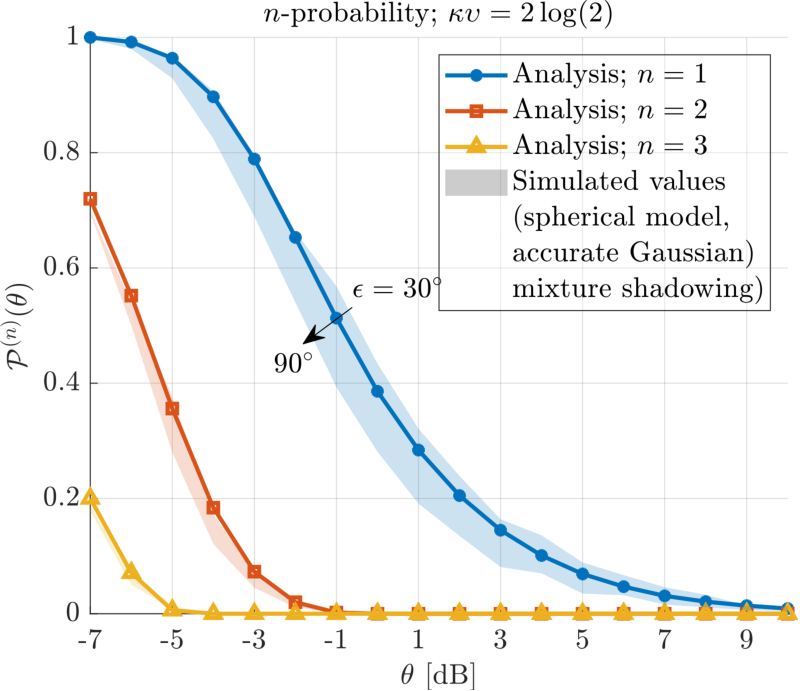
\includegraphics[width=\linewidth]{nprobability.pdf}
  \caption{The $n$-probabilities for $\kappa v=2 \log(2)$ (the average number of effective UEs inside a $-3$ dB footprint). 
} 
  \label{fig:nprobability}
\end{figure}


  
\begin{figure}[h]
  \centering
  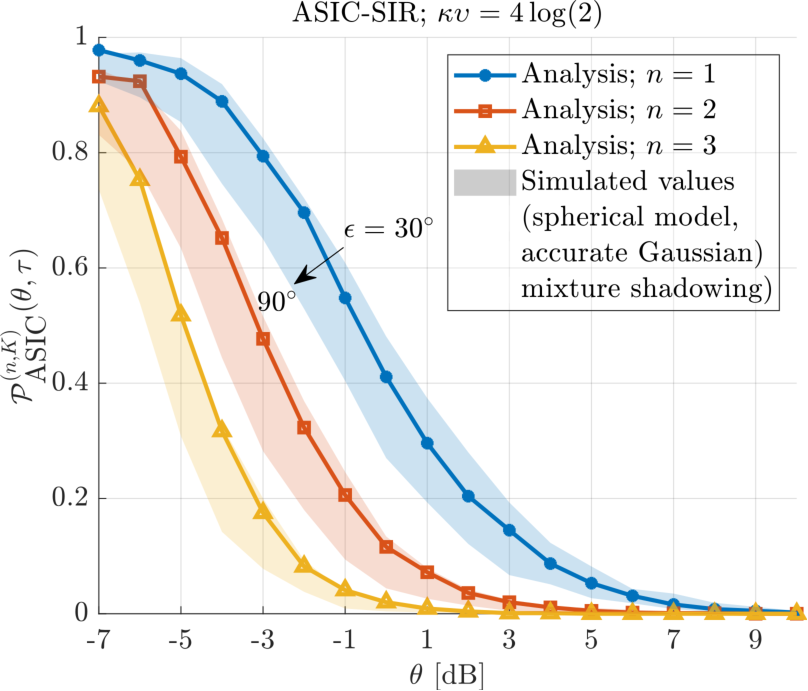
\includegraphics[width=\linewidth]{ASICSIR.pdf}
  \caption{The SIC-SIR for doubling the {average number of effective UEs inside the $-3$ dB footprints} compared to Figure \ref{fig:nprobability}; $\kappa \upsilon = 4 \log(2)$.} 
  \label{fig:ASICSIR}
\end{figure}


Figures \ref{fig:nprobability} and \ref{fig:ASICSIR} depict the $n$-probabilities \eqref{eq:kprobability} and SIC-SIR for $\tilde{\kappa}\upsilon=2$ and  $\tilde{\kappa}\upsilon=4$ \eqref{eq:SICprob} with $K=3$, respectively. We use the values presented in Table \ref{table:parameters} in the simulations. However, the crucial system parameter is $\tilde{\kappa}\upsilon$. Hence, for example, instead of scaling $\lambda$, we could adjust the width of the antenna gain for each elevation angle according to \eqref{eq:upsilon} and \eqref{eq:kappa} to match the corresponding $\tilde{\kappa}\upsilon\equiv{\kappa}\upsilon/\log(2)$.

The figures illustrate that SIC-SIR can achieve comparable coverage probabilities for the strongest UE within the region $\theta \in (-7,10)$ dB while doubling the average number of effective UEs inside a $-3$ dB footprint, denoted as $\kappa \upsilon$. Additionally, the performance of the $2$\textit{nd} and $3$\textit{rd} UEs is significantly enhanced. Consequently, a single LEO BS could potentially serve multiple UEs effectively.

Further, similar to \eqref{eq:SIR2}, we can calculate an upper bound for the variance of the SIR of the strongest signal before interference cancellation for $\tilde{\kappa} \upsilon = 4$: $\text{var}(\text{SIR}_{1,[1]}) =\mathbb{E}(\text{SIR}^2_{1,[1]})-\mathbb{E}(\text{SIR}_{1,[1]})^2  \leq 1.2$. This represents a significant improvement compared to the infinite variance for $\tilde{\kappa} \upsilon = 2$. 

We conclude that interference cancellation, particularly successive interference cancellation (SIC), is a viable solution for mitigating the considerable variability in link quality experienced by users in a narrow-beam low Earth orbit (LEO) uplink. These findings are also relevant to the downlink, given that the LEO footprint locations follow a Poisson distribution on the Earth's surface.






%% \begin{verbatim}
%% \begin{table}
%% \begin{center}
%% \caption{Filter design equations  ...}
%% \label{tab1}
%%     \begin{tabular}{| c | c | c |c|}
%%       \hline
%%       & $\mathcal{P}^{(1)}(\cdot)$& $\mathcal{P}^{(2)}_{\text{IC}}(\cdot)$& $\mathcal{P}^{(2)}_{\text{SC}}(\cdot)$\\
%%       \hline
%%       $\mathbb{E}(\cdot)$&$1.4$ & $1.4$ &$1.4$\\ 
%%       \hline
%%       $\tilde{\kappa}$& $2/\upsilon_{} $ &$2.6/\upsilon_{}$& $3.4/\upsilon_{}$\\
%%       \hline
%%       Var$(\cdot)$& $\infty$ & $2.6$ &$2.3$\\
%%       \hline 
%%     \end{tabular}
%% \end{center}
%% \end{table}
%% \end{verbatim}








\bibliographystyle{IEEEtran}
%\bibliography{IEEEabrv, bib}
\bibliography{IEEEabrv,source}


\end{document}
 
